\section{Methodology}
Testing a model's ability to generate query execution plans requires two resources, a running model and a real database for sourcing queries, execution plans, and database statistics. Since any moderately-sized database would suffice, we recycled a database for university attendance from a past publication \cite{hybl2023}. In the following subsection, we explain the setup required for our database and how we obtained the necessary data for the project. Then, in the next subsection, we explain the code used for the inference experiments.

\subsection{Model Input}
We hypothesized that an LLM would require two types of input to generate an execution plan: database descriptors and the query to be optimized. We obtained both from a database server we ran locally using \lstinline{mssql} docker containers. To set up the docker container, we ran \lstinline{docker-compose -f sauAttendance.yml up -d} where \lstinline{sauAttendance.yml} is the file shown in Listing \ref{lst:sauAttendance.yml}. This spins up a local container that we can connect to through SQL Server Management Studio (SSMS) using the host \lstinline{localhost,1433}, the user \lstinline{sa}, and the password specified in the \lstinline{yml} file. Using \lstinline{docker-compose} preserves the database even if the container is destroyed and recreated.

\begin{lstlisting}[
  language=yaml,
  style=lightBlock,
  caption={sauAttendance.yml file used with \lstinline{docker-compose}},
  label={lst:sauAttendance.yml}
]
version: '3.8'

name: sau-db
services:
  mssql:
    container_name: attendanceDB
    image: mcr.microsoft.com/mssql/server
    environment:
      ACCEPT_EULA: "Y"
      SA_PASSWORD: "myStrongPassword"
    ports:
      - 1433:1433
    volumes:
      - mssql_attendanceDB:/var/opt/mssql
volumes:
  mssql_attendanceDB:
\end{lstlisting}

Once running, we constructed a relational database by importing comma-separated values (CSV) files from a past project \cite{hybl2023} into the database using SSMS. Primary and foreign keys were also configured in SSMS. The resulting schema for this database can be seen in Figure~\ref{fig:schema}. All entities are transitively related using primary/foreign keys.
\begin{figure*}[ht]
  \centering
  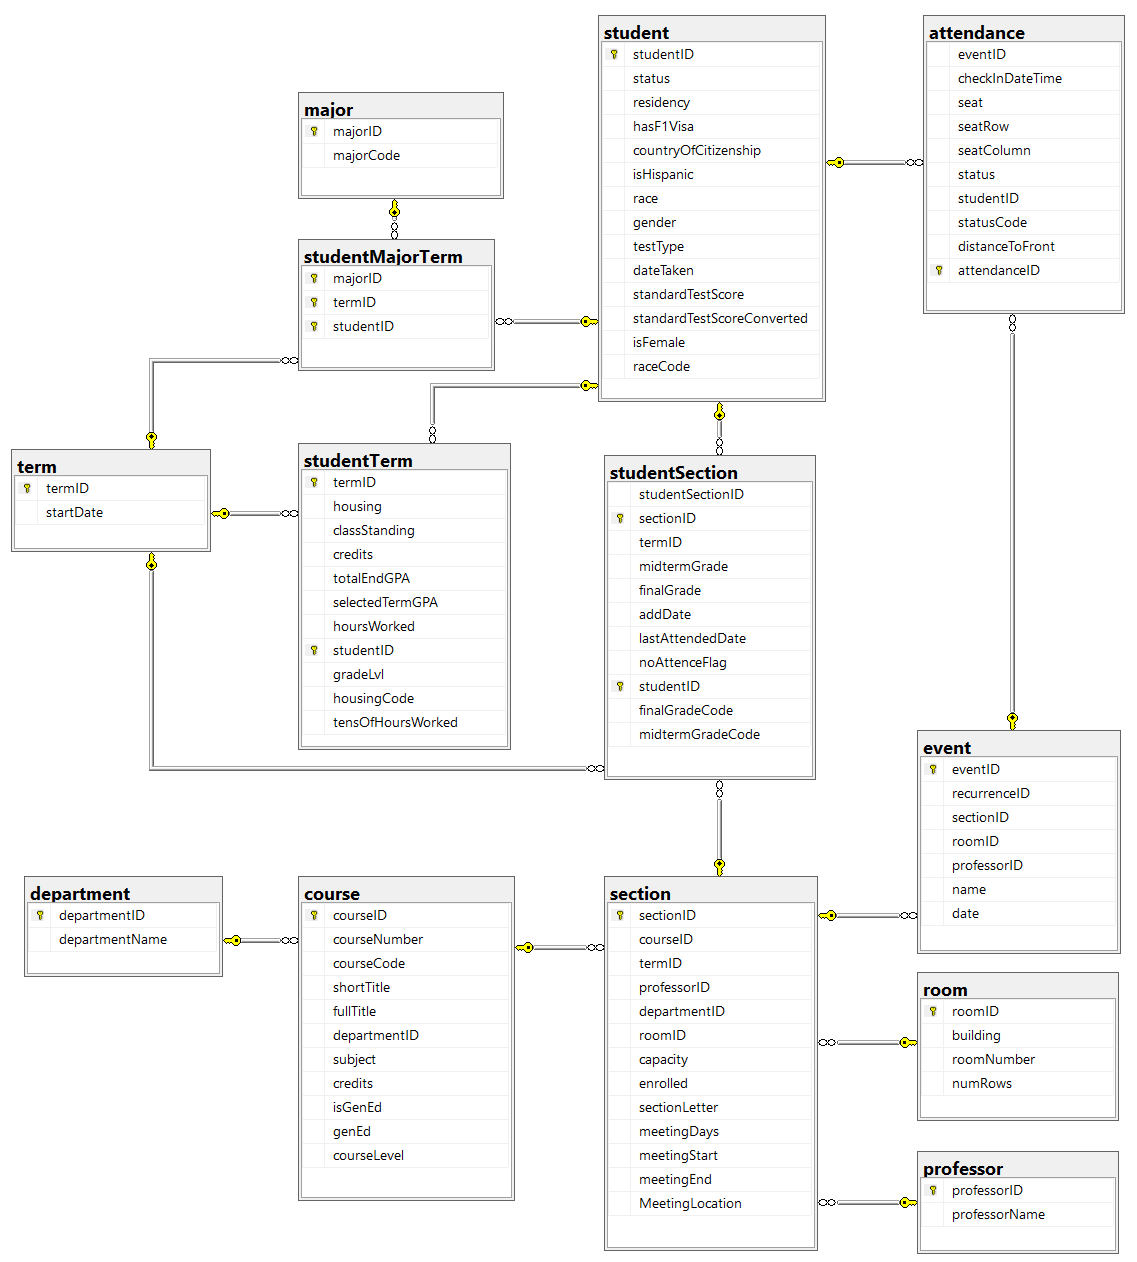
\includegraphics[width=\textwidth]{figures/attendanceDBSchema.png}
  \caption{The database schema as visualized by Microsoft SQL Server Management Studio.}
  \label{fig:schema}
\end{figure*}

\subsubsection{Queries}
With the data available, queries can be written. All queries were written manually to ensure quality, correctness, and diversity. For example, consider the queries in Listings \ref{lst:selectCSPhysDept} and \ref{lst:selectNursBioDept}. The series of operations provided by SQL server for both of these examples comprise the following steps (cleaned for visual appearance):

\begin{enumerate}
  \raggedright
  \item Clustered Index Seek((professor AS p), ordered forward)
  \item Clustered Index Scan(section AS s)
  \item Clustered Index Seek((department AS d),  where:(d.departmentName = 'firstDepartmentName' OR d.departmentName = 'secondDepartmentName') ordered forward)
  \item Clustered Index Scan(course AS c)
  \item Nested Loops(Inner Join, outer refs:(c.departmentID))
  \item Hash Match(Inner Join, Hash:(c.courseID) = (s.courseID))
  \item Nested Loops(Inner Join, outer refs:(s.professorID))
\end{enumerate}

\begin{lstlisting}[
  language=SQL,
  style=sqlStyle,
  caption={SQL query that selects professors who taught in the computing and physics departments.},
  label={lst:selectCSPhysDept}]
  select p.professorName from professor p join section s on p.professorID = s.professorID join course c on s.courseID = c.courseID join department d on c.departmentID = d.departmentID where d.departmentName = 'Computing' or d.departmentName = 'Physics';
\end{lstlisting}

\begin{lstlisting}[
  language=SQL,
  style=sqlStyle,
  caption={SQL query that selects professors who taught in the nursing and biology departments.},
  label={lst:selectNursBioDept}]
  select p.professorName from professor p join section s on p.professorID = s.professorID join course c on s.courseID = c.courseID join department d on c.departmentID = d.departmentID where d.departmentName = 'Nursing' or d.departmentName = 'Biology';
\end{lstlisting}

Aside from the names of the departments, these two queries require identical procedures to retrieve. Because we are interested in what the LLM's method of information retrieval actually is, the queries presented to it should require diverse operations to execute. The query in Listing \ref{lst:selectAvgCourseCredits} would be a more appropriate example because it's execution plan includes sort, order by, stream aggregation, group by, and compute scalar functions.

\begin{lstlisting}[
  language=SQL,
  style=sqlStyle,
  caption={SQL query that gets the average course credits in each department.},
  label={lst:selectAvgCourseCredits}]
  select d.departmentName, avg(c.credits) as 'creditAverage' from course c join department d on c.departmentID = d.departmentID group by d.departmentName;
\end{lstlisting}

With these goals for queries in mind, \dataRows diverse queries were written and executed on the database in Figure \ref{fig:schema}. Obtaining query execution plans merely requires turning on the \lstinline{showplan_text} setting in the SQL server. We can achieve this by executing \lstinline{set showplan_text on;}. With this setting, SSMS returns execution plans instead of the results of a query.

However, the execution plans are unnecessarily messy. For example, the beginning of the raw execution plan for Listing \ref{lst:selectCSPhysDept} includes the unnecessary syntax shown in Text \ref{text:messyExecPlan}. The indentation, pipes, extra parentheses, and extra words such as \lstinline{OBJECT} are distracting and would never be required as output from a large language model that was part of a database. Thus, we chose to clean this data to make it more human readable.

\begin{text}
  \begin{verbatim}
|--Nested Loops(Inner Join, OUTER
  REFERENCES:([s].[professorID]))
|--Hash Match(Inner Join, HASH:
  ([c].[courseID])=([s].[courseID]))
|    |--Nested Loops(Inner Join,
  OUTER REFERENCES:([c].[departmentID]))
|    |    |--Clustered Index Scan(
  OBJECT:([attendanceDB].[dbo].[course].
  [PK_course] AS [c]))
SEEK:([d].[departmentID]=[attendanceDB].
[dbo].[course].[departmentID] as [c].
[departmentID]),  WHERE:([attendanceDB].
[dbo].[department].[departmentName] as 
[d].[departmentName]=N'Computing' OR
[attendanceDB].[dbo].[department].
[departmentName] as [d].[departmentName]
=N'Physics') ORDERED FORWARD)
. . .\end{verbatim}
  \caption{Execution plan output by SSMS}
  \label{text:messyExecPlan}
\end{text}

The execution plan cleaning procedure was automated with a simple script in \lstinline{sqlPlanCleaner.py}. Listing \ref{lst:sqlPlanCleaner} shows this script. It begins by removing pipes, brackets, parentheses, and unnecessary identifiers. It then filters out tokens such as \lstinline{residual}, \lstinline{define}, \lstinline{opt_bitmap}, and \lstinline{object} because these functions or objects are never the ``main'' function of any step in the queries we planned to test. Next, the \lstinline{N} preceding all string literals (such as in \lstinline{N'Computing'}) and any unnecessary parentheses are removed. Some execution plans also contained empty functions nested inside top-level operations, so these were removed. Finally, the output is numbered and placed on one line so it can be stored as a column in a CSV file.

\begin{lstlisting}[
  language=python,
  style=fullPython,
  caption={Data cleaning with the \lstinline{cleanPlan} function},
  label={lst:sqlPlanCleaner}
]
import re
def cleanPlan(query: str) -> str:
  # 1. rm square brackets
  query = re.sub(r'\[([^\]]+)\]', r'\1', query)
  # 2. rm unnecessary syntax
  query = re.sub(r'[ \t]*(\|(--)?)|(sauAttendance\.dbo\.)', '', query)
  query = re.sub(r'attendanceDB\.dbo\.([a-zA-Z]+)\.PK__?[a-zA-Z]+(?:__)?\w*', r'\1', query)
  query = re.sub(r'attendanceDB\.dbo\.(\w+) as (\w+)', r'\1 as \2', query)

  # 3. remove unnecessary entities
  query = re.sub(r',? *residual:.*?define:.*?\)', '', query, flags = re.I)
  query = re.sub(r',? *opt_bitmap\d+,?', '', query, flags = re.I)
  query = re.sub(r'object:', r'', query, flags = re.I)
  # 4. clean up 'N' in front of strings
  query = re.sub(r"N('[^']+')", r'\1', query, flags = re.I)
  # 5. rm multiple parentheses
  query = re.sub(r'\(\(([^)]+)\)\)', r'(\1)', query)
  # 6. rm empty f(x)s
  query = re.sub(r',?[a-zA-Z]+:\(\)', r'', query)
  
  # 7. reverse and rm line breaks
  steps = query.split('\r\n')[::-1]
  steps = [f'{num + 1}: {q}' for num, q in enumerate(steps)]
  query = '\\n# '.join(steps)
  query = '# ' + query
  return query
\end{lstlisting}

\subsubsection{Database Information}
To generate an execution plan, any system would require information about the database schema. We provided this information as part of the system prompt to the model. As shown in Text \ref{text:sysPrompt}, the system prompt consists of instructions for the model, a thorough description of the database, and an example of its input and output. The full system prompt can be viewed \href{https://github.com/MatousAc/llamaExecPlan/blob/main/src/sysPrompt.txt}{here}.

\begin{text}
  You are an AI that produces execution plans for a relational database. Description of database. Here are the tables:\\
  \\
  Table: tableName Cardinality: \#\#\#\#\#\\
  PK: pkColumnName\\
  column2Name\\
  column3Name\\
  ...\\
  Output instructions. Suggested functions to use in output. Example:\\
  Query: example query\\
  Execution Plan:\\
  1: Function(arg)\\
  2: Function2(arg2)
  \caption{The structure of the system prompt provided to the model.}
  \label{text:sysPrompt}
\end{text}

\subsection{Model Operation}
The next step is to prompt the LLM with a query and database description. Our suite of Python scripts and configuration files orchestrates the entire process, from configuring the system and formatting data to performing inference and logging results. See Figure \ref{fig:classDiagram} for a class diagram.
\begin{figure}[htb]
  \centering
  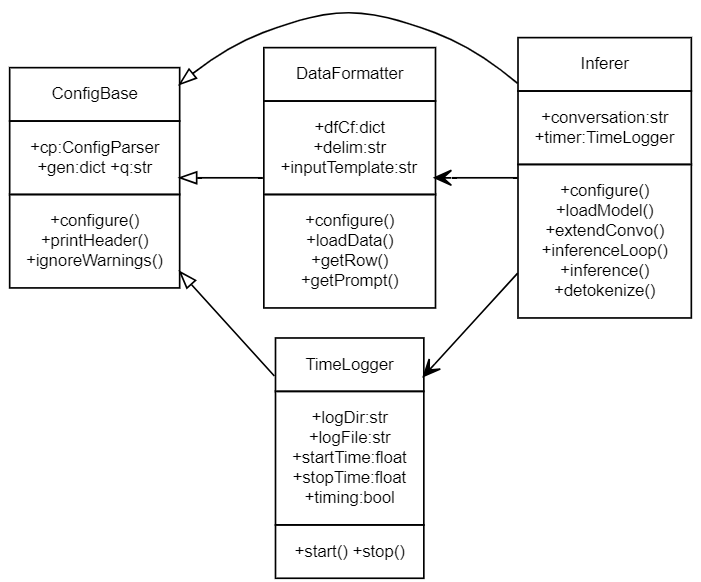
\includegraphics[width=0.48\textwidth]{figures/classDiagram.png}
  \caption{A UML diagram of the classes used in this experiment.}
  \label{fig:classDiagram}
\end{figure}

The first core component is the configuration base class, \lstinline{configBase.py}, which centralizes the management of system settings and paths as defined in the \lstinline{config.ini} file, ensuring a flexible and adaptable environment for different experimental setups. Listing \ref{lst:configBase} contains an example from \href{https://github.com/MatousAc/llamaExecPlan/blob/main/src/configBase.py}{configBase.py}. Notice the \lstinline{configure} function that is called but does nothing. This function is meant to be overriden in derived classes, but will still be automatically called upon object construction.

\begin{lstlisting}[
  language=Python,
  caption={The loadModel function.},
  label={lst:configBase}
]
import os, sys
from configparser import ConfigParser

class ConfigBase:
  def __init__(self, configFilePath):
    base = os.path.normpath(os.getcwd())
    self.cp = ConfigParser()
    self.cp.read(configFilePath)

    self.paths = self.cp['paths']
    for path in self.paths:
      # prepend base to each path
    
    # set up general other configuration
    self.gen = self.cp['general']
    self.q = self.gen['q'] == 'True'
    self.configure()
  
  def configure(self):
    pass
\end{lstlisting}

The \lstinline{Inferer} class takes center stage by loading the LLM and its tokenizer and facilitating the inference process. These operations are shown in Listing \ref{lst:inferer}. The \lstinline{Inferer} requests query examples from the \lstinline{DataFormatter} and then formats prompts for the LLM. It also manages the iterative conversation with the model, ensuring that after each query is processed only the output is appended to the growing conversation.
\begin{lstlisting}[
  language=Python,
  style=fullPython,
  caption={loadModel},
  label={lst:inferer}
]
def loadModel(self):
  # quantized LoRA (QLoRA) - uses 4-bit normal float to lighten GPU/CPU load
  self.bnbConfig = BitsAndBytesConfig(
    load_in_4bit = True,
    # we leave the model quantized in 4 bits
    bnb_4bit_quant_type = 'nf4',
    bnb_4bit_compute_dtype = torch.float16
  )
  # load our model
  self.model = AutoModelForCausalLM.from_pretrained(
    pretrained_model_name_or_path=self.paths['model'],
    quantization_config=self.bnbConfig,
    device_map='auto'
  )
  self.model.config.use_cache = False

  # load tokenizer
  self.tokenizer = AutoTokenizer.from_pretrained(self.paths['model'])
  self.tokenizer.pad_token = self.tokenizer.eos_token

def inference(self):
    nextPrompt = self.dataFormatter.getPrompt()
    self.extendConversation(nextPrompt)
    modelInput = self.tokenizer(self.conversation, return_tensors='pt').to('cuda')

    self.timer.start()
    self.model.eval()
    with torch.no_grad(): # grad only used in training
      tokens = self.model.generate(**modelInput, max_new_tokens=100)[0]
      response = self.tokenizer.decode(tokens, skip_special_tokens=True)
      response = response.split('[/INST]')[-1]
      self.timer.stop()
      self.conversation += response
      print(f'Llama: {response}')

if __name__ == '__main__':
  trainer = Inferer()
  trainer.loadModel()
  trainer.inference()
\end{lstlisting}

The \lstinline{DataFormatter} class, on the other hand, provides the \lstinline{Inferer} prepare and format SQL queries from a dataset, creating prompts that are fed into the LLM. When the Inferer. This preparation involves embedding queries within a structured template (taken from \lstinline{config.ini} and shown in Text \ref{text:inputTemplate}) that guides the LLM's generation process, aiming for consistency and relevance in the generated execution plans.
\begin{text}
  inputTemplate: $<$s$>$ \#\#\# Create a query execution plan for an RDBMS for the following query: \#\#\# Query: $<$query$>$ \#\#\# Execution Plan: $<$execPlan$>$
  \caption{Model prompt template}
  \label{text:inputTemplate}
\end{text}

Finally the \lstinline{TimeLogger} class provides performance metrics alongside the \lstinline{Inferer} class by timing the inference process. This offers insights into the efficiency of the model under various conditions.

Using the \lstinline{Inferer}'s \lstinline{inference()} function and its dependencies, our experiments can be run by simply modifying the input template in \lstinline{config.ini} and then testing inference using \lstinline{python inferer.py}.

This hierarchical but compartmentalized architecture not only enables the systematic generation of execution plans by the LLM but also provides a framework for evaluating the model's performance and effectiveness in optimizing SQL queries. Through this setup, we are able to easily prompt the model to explore the potential of LLMs in automating and enhancing query execution plans, contributing to the broader field of applying machine learning techniques to database optimization and management.

